
 \documentclass[18pt,a4paper]{report}
 
 \usepackage[pagebackref=false,colorlinks,linkcolor=blue,citecolor=magenta]{hyperref}
 
 \usepackage[nottoc]{tocbibind}
 \usepackage{calc}
 \usepackage{eso-pic}
 \usepackage{hyperref}
 \usepackage {fancybox}
 \usepackage{graphicx, xcolor}
 
 \usepackage{xepersian}
 \settextfont{B Nazanin}
 \title{نگاهی به برندگان جایزه  \lr{Loebner}}
\author{ آقایان محمدرضا محمدی، امیر محمدی و رضا رضایی}
\renewcommand{\bibname}{مراجع}
\begin{document}


	
 	\maketitle
 	\tableofcontents
 	
 	
 	\chapter{جایزه \lr{Loebner} چیست؟} 
 	هر ساله یک رقابتی در زمینه هوش مصنوعی برگزار میشود که در آن جوایزی به برنامه های کامپیوتری اهدا میشود که از نظر داوران،  شبیه ترینِ به انسان هاست. قالب این مسابقه ها بر اساس یک تست استاندارد تورینگ هست. در هر دور، یک قاضی انسانی همزمان مکالمه های متنی را با یک برنامه کامپیوتری و یک انسان از طریق کامپیوتر برگزار میکند، بر اساس پاسخ های دریافت شده، قاضی باید تصمیم بگیرد که کدام، کدام است!!!
 	
 	\large{\textbf{در زیر لیستی از برندگان جایزه \lr{loebner}  را مشاهده میکینم: }}
 	
 	\begin{LTR}
 		\begin{center} 
 			\begin{tabular}{lclclcl} 
 				
 				\\ \lr{\textbf{Year}} & \lr{\textbf{Winner}} & \lr{\textbf{Program}}
 				\vspace{10pt}
 				
 				
 				\\ \lr{2000} & \lr{Richard Wallace} & \lr{Artificial Linguistic Internet Computer Entity (A.L.I.C.E.)}
 				
 				\\ \lr{2001} & \lr{Richard Wallace} & \lr{Artificial Linguistic Internet Computer Entity (A.L.I.C.E.)}
 				
 				\\ \lr{2002} & \lr{Kevin Copple}    & \lr{Ella}
 				
 				\\ \lr{2003} & \lr{Juergen Pirner}  & \lr{Jabberwock}
 				
 				\\ \lr{2004} & \lr{Richard Wallace} & \lr{Artificial Linguistic Internet Computer Entity (A.L.I.C.E.)}
 				
 				\\ \lr{2005} & \lr{Rollo Carpenter}    & \lr{George (Jabberwacky) }
 				
 				\\ \lr{2006} & \lr{Rollo Carpenter}    & \lr{Joan (Jabberwacky) }
 				
 				\\ \lr{2007} & \lr{Robert Medeksza}    & \lr{Ultra Hal}
 				
 				\\ \lr{2008} & \lr{Fred Roberts}    & \lr{Elbot}
 				
 				\\ \lr{2009} & \lr{David Levy}    & \lr{Do-Much-More}
 				
 				\\ \lr{2010} & \lr{Bruce Wilcox}    & \lr{Suzette }
 				
 				\\ \lr{2011} & \lr{Bruce Wilcox}    & \lr{Rosette}
 				
 				\\ \lr{2012} & \lr{Mohan Embar}    & \lr{Chip Vivant}
 				
 				\\ \lr{2013} & \lr{Steve Worswicky}    & \lr{Mitsuku}
 				
 				\\ \lr{2014} & \lr{Bruce Wilcox}    & \lr{Rose}
 				
 				\\ \lr{2015} & \lr{Bruce Wilcox}    & \lr{Rose}
 				
 				\\ \lr{2016} & \lr{Steve Worswick}    & \lr{Mitsuku}
 				
 				\\ \lr{2017} & \lr{Steve Worswick}    & \lr{Mitsuku}
 				
 				\\ \lr{2018} & \lr{Steve Worswick}    & \lr{Mitsuku}
 				
 				\\ \lr{2019} & \lr{Steve Worswick}    & \lr{Mitsuku}
 				
 				
 				
 			\end{tabular}
 		\end{center}
 	\end{LTR}
 	
 	
 	\section{\lr{Loebner} کیست؟}
 	هیو لوبنر متولد 26 مارس 1942 و وفات 4 دسامبر 2016 به عنوان حامی جایزه لوبنر و تجسم آزمون تورینگ مشهور بود. او یک مخترع آمریکایی دارای 6 اختراع و یک فعال اجتماعی آشکار برای جزم زدایی فحشا بود.
 	
 	
 	
	 \chapter{برندگان جایزه \lr{loebner}}
	 
	

	 \section{\lr{Steve Worswick}}
 	استیو وورسویک، سازنده برنامه \lr{Mitsuku} توانسته است در سال های 2013، 2016، 2017، 2018 و 2019 جایزه لوبنر را از آن خود کند. \lr{Mitsuku} یک ربات چت هست که از فن آوری \lr{AIML} استفاده میکند. \lr{Mitsuku}  به عنوان یک بازی فلش در بازی های \lr{Mousebreaker}  و در فیسبوک مسنجر، چت گروهی \lr{Telegram} \lr{Twitch} و \lr{Kik} با نام کاربری "\lr{Pandorabots}" موجود است و با همین نام در اسکایپ نیز در دسترس بود اما توسط توسعه دهنده آن حذف شد.
 	
\begin{figure}
	\begin{center}
		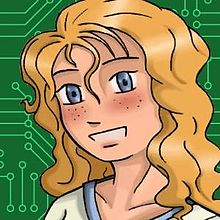
\includegraphics[width=5cm, height=5cm]{imgs/Mitsuku.jpg}
		\label{Mitsuku image}
		\caption{\lr{One of Mitsuku's avatars}}
	\end{center}
\end{figure} 	
 	
 برنامه 	\lr{Mitsuku} ادعا میکند که یک زن 18 ساله از شهر لیدزِ انگلیس هست. این شامل کلیه پرونده های \lr{AIML} آلیس هست، با تعداد بسیاری از اضافات مکالمات ایحاد شده توسط کاربر و همیشه یک کار در حال انجام هست. \lr{Worswick} ادعا میکند که از سال 2005 در این زمینه کار کرده است. 
  
 هوش \lr{Mitsuku} توانایی پاسخ دهی به موضوعات خاص را دارد. به عنوان مثال اگر شما از او بپرسید: "میتوانی خانه بخوری!؟" او به دنبال صفت هایی از خانه میگردد و با یافتن صفت "ساخته شده از" با برخورد با مقدار "آجر" پاسخ خواهد داد "نه!"، چرا که یک خانه خوردنی نیست. او میتواند بازی کند و کارهای شگفت انگیزی به درخواست کاربر انجم دهد. در سال 2015 به طور میانگین او یک چهارم میلیون بار مکالمه کرد. 
 


 \section{\lr{David Levy}}
دیوید لوی متولد ۱۹۴۵، استاد بین‌المللی شطرنج که شهرت عمده وی به دلیل مشارکت در پروژه های هوش مصنوعی مرتبط با شطرنج می‌باشد.
وی در سال‌های ۱۹۹۷ و ۲۰۰۹ برنده جایزه لوئبنر شده است.	 

\section{\lr{Rollo Carpenter}}
رولو کارپنتر (متولد ۱۹۶۵)، محقق هوش مصنوعی و خالق \lr{Jabberwacky} و \lr{Cleverbot} که در سال‌های ۲۰۰۵ و ۲۰۰۶ و ۲۰۱۰ برنده جایزه لوئبنر شده است.
\lr{Jabberwacky} یکی از اولین چت‌بات های شبیه‌ساز مکالمات انسان می‌باشد که به گفته آقای کارپنتر، همانطور یاد ‌میگیرد که یک انسان واقعی چیزی را یاد می‌گیرد؛ این روبات با استفاده از سیستم الگویاب فازی می‌تواند عبارات پیچیده و مفهومی را هم متوجه شده و به آنها پاسخ دهد.
 
 \section{\lr{Bruce Wilcox}}
 بروس ویلکاکس یک حرفه ای در حوزه \lr{chatbot} هست. طی 7 سال گذشته، ربات های او بیش از سایر رقبا در در مسابقات لوبنر در رده های 1 یا 2 قرار گرفته اند. یکی از چت بات های اصلی کخ جوایز زیادی از لوبنر را برای بروس ارمغان آورده است، \lr{Rose} است.
 
 برجسته ترین نکته در مورد بروس این است که وی نسبت به تقریباً هر مهندس و دانشمند دیگری در جهان عمیقاً درباره رابطهای مکالمه فکر کرده است و مواردی را واقعاً شسته و رفته ساخته است.او حتی تا آنجا پیش رفت که زبان و موتور نوشتاری خود ، \lr{ChatScript} را ایجاد کرد. او و همسرش سو یک شرکت پردازش زبان طبیعی \lr{Brillig Understanding} را اداره کردند ، جایی که در مورد پروژه ها مشورت می کنند و \lr{ChatScript} را تبلیغ می کنند. 

 	\begin{center}
 		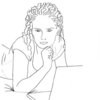
\includegraphics[width=5cm, height=5cm]{imgs/chatbot_rosette_d____10513.jpg}
 		\label{Rose image}

 	\end{center}

 
 برنامه \lr{Rose } خود را یک هکر کامپیوتری 20 ساله اهل سانفرانسیسکو معرفی میکند.این برنامه به عنوان \lr{Rosette}  در سال 2011 برنده جایزه لوبنر شد و در سال 2014 به عنوان \lr{Rose} .
 
  
 \section{\lr{Mohan Embar}}
 موهان امبار در سال ۲۰۱۲ برای \lr{Chip Vivant} برنده جایزه لوئبنر شد.
 روبات \lr{Chip Vivant} بر خلاف اکثر چت‌بات‌ها به جای استفاده از دیتابیسی عظیم از پاسخ‌های قبلا تعیین شده، با استقرا و منطق به گفته‌های کاربر پاسخ می‌دهد.

\section{\lr{Richard Wallace}}
در سال 2000 جایزه لوبنر به دکتر ریچارد والاس که یک نویسنده امریکایی است تعلق می گیرد او متولد سال 1960 در پورتلند می باشد و بنیا گذار بنیاد هوش مصنوعی \lr{A.L.I.C.E  }که مخفف کلمه \lr{Artificial Linguistic Internet Computer Entity }به معنی نهاد رایانه ای اینترن زبان مصنوعی است می باشد در مورد این کلمه در ادامه توضیحاتی بیان خواهد شد , کار دکتر والاس در زد دی تی وی ، سی ان ان ، نیویورک تایمز و نشریات متعدد دیگر ظاهر شده است والاس کار خود را در سال 1995با \lr{ALICE}  شروع کرد و در سال های 2000 ، 2001 و 2004 جایزه لوبنر را دریافت کرد.  

\lr{Internet Linguistic Internet Computer} که با نام \lr{Alicebot} یا به صورت ساده تر آلیس شناخته میشود یک گفتگوی پردازش زبان طبیعی است این برنامه به صورت الهام گرفته شده از برنامه الیزا جوزف کلاسیک می باشد .
این برنامه با استفاده از برخی قوانین تطبیق الگوهای اکتشافی به گفتگو با انسان می پردازد اما نکته جالب در مورد این برنامه این است که نمی تواند آزمون تورینگ را بگذراند و دلیل آن هم این است که کاربر معمولی معمولا در طول مکلمات نچندان بلند جنبه های مکانیکی خود را نشان می دهد.

آلیس در آغاز به وسیله دکتر ریچارد والاس تشکیل شده است این برنامه از یک طرح \lr{XML}  به نام \lr{AIML}   یا همان زبان نشانه گذاری هوش مصنوعی برای تعیین قوانین گفتگوی اکتشافی استفاده می کند کد برنامه الیس به صورت منبع ازاد در گیت هاب دکتر والاس در دسترس می باشد این برنامه در اغاز سال 1998 یعنی در آغاز جاوا بازنویسی شد که تجسم اجرای جاوا برنامه D  است. این برنامه با الهام از اینکه آیا انسان می تواند با یک ربات وارد رابطه شود و با او رابطه برقرار کند برگرفته شده است و الایس سعی می کند با گفتگو این کار را انجام دهد چون یک ربات چت است .

\section{\lr{Kevin Copple}}
الا "\lr{Ella}" که در سال 2002 برنده جایزه لوبنر شد یک ربات شوخ است که او از پایگاه داده ای استفاده می کند که شامل هزاران شوخی،حکایت،شعر و ... می شودکه به الا کمک مکند تامکالمات اموزنده و جالبی با انسان داشته باشداین اسیتم برای افزایش دانایی خود و اثر بخشی نظر شما را در مورد جوک ها و تصاویر و چیز های دیگر می پرسد .الا در سال 200 ایجاد شده استو تخصص او زبان طبیعی است او ویژگی هایی مثل توانایی بازی کردن دارد الا در سال 2001 در مسابقات لوبنر نایب قهرمان شد اما در سال 2002 توانست رتبه اول را کسب کند .

\section{\lr{Juergen Pirner}}
یورگن پیرنر متولد سال1956 در آلمان است این شخ در سال 2003 بابت \lr{Jabberwock}  برنده جایزه لوبنر شد یورگن در شهر هامبورگ آلمان زندگی می کند ، او اثر خود را با الگو برداری از \lr{Jabberwocky} از شعر لوییس کارول به همین نام خلق کرده است .

جابر وک "\lr{jabberwock}" یک هوش مصنوعی از نوع چت بات ها است که توانایی درک بیش از 30000 کلمه را دارد ونکته بسیار هجان انگیز این است که در حدود 22000000 جمله را می داند انسان می تواند درباره هر موضوعی با جابر به صحبت بنشیند 
این برنامه شبیه سازی چت طبیعی انسان به شیوه جالب سرگرم کننده و طنز آمیز است هدف اعلام شده این پروژه ایجاد یک هوش مصنوعی است که قادر به گذراندن آزمون تورینگ است. این برنامه برای تقلید از تعامل انسان و انجام گفتگو با کاربران طراحی شده است و برای انجام کارکردهای دیگر طراحی نشده است.



\begin{thebibliography}{9}
	\latin
	\bibitem{Mitsuku}
	\lr{https://en.wikipedia.org/wiki/Mitsuku}
	
	\bibitem{DavidLevy}
	\lr{https://en.wikipedia.org/wiki/David\_Levy}
	
	\bibitem{RolloCarpenter}
	\lr{https://en.wikipedia.org/wiki/Rollo\_Carpenter}
	
	\bibitem{ChipVivant}
	\lr{http://www.chipvivant.com}
	
	\bibitem{Rose}
	\lr{https://chatbotsmagazine.com/rose-in-the-loebner-chatbot-competition-an-interview-with-bruce-wilcox-eac0a8b61647}
	
	\bibitem{Richard wallace}
	\lr{ https://en.wikipedia.org/wiki/Richard-Wallace-(scientist) }
	
	\bibitem{Juergen pirner}
	\lr{ https://en.wikipedia.org/wiki/Juergen-Pirner}
	
\end{thebibliography}
 	
 
 	
\end{document}
